\chapter[Estado del arte]{Estado del arte, requisitos y arquitectura}
\label{sec:state_of_art}

\section{Virtualización de servidores}
\label{subsec:virt_servers}

Como ya dije antes, la virtualización aplicada a servidores no es nada que haya surgido los últimos años. Pero cuando IBM comenzó a trabajar con los primeros \emph{mainframes} concurrentes, su propósito era meramente ofrecer a sus usuarios una manera de trabajar al mismo tiempo en un mundo que, en aquellos tiempos, era puramente secuencial.

Hoy en día la virtualización ha ido evolucionando gradualmente, resultando en diferentes técnicas y métodos que permiten sustituir de manera eficaz y flexible las máquinas físicas. Cada método funciona de una manera diferente, con sus ventajas y desventajas, que iré explorando brevemente en las siguientes secciones:

\subsection{Cómo opera el instituto actualmente}
\label{subsubsec:virt_des}

Antes de discutir los pros y los contras de los diferentes métodos de virtualizacion, veamos cómo se ofrecen los servicios actualmente: en una máquina personalizada con las siguientes características:

\begin{itemize}
    \item \textbf{CPU:\@ }Intel Xeon E-1220 @ 3.10 GHz
    \item \textbf{RAM:\@ }8 GB
\end{itemize}

Considerando los servicios ofrecidos (Un par de servidores web con la página web del centro y un Owncloud, y un servidor DHCP.), ésta máquina está lo suficientemente preparada para dichos servicios, pero opino que se pueden ofrecer de manera más eficiente. A continuación, listaré los que a mi juicio son los principales detrimentos de éste sistema:

\begin{itemize}
    \item \textbf{Aprovechamiento mínimo de recursos: }Aunque ésto se vea atenuado de cierto modo en este caso, los recursos de una máquina raramente se aprovechan del todo, ya que un servicio no hará uso de todo el hardware disponible.

    \item \textbf{Ningún tipo de aislamiento entre servicios: }Debido a que todos los servicios se están ejecutando en el mismo sistema operativo sin ningún mecanismo de aislamiento, cualquier problema grave en cualquiera de los servicios podría comprometer la disponibilidad de los otros servicios.

    \item \textbf{Costos de expansión: }Expandir ésta arquitectura puede resultar muy costoso, tanto en materia de hardware, electricidad, y acondicionamiento de la sala de servidores.
\end{itemize}

\subsection{Ventajas de la virtualización}
\label{subsec:virt_servers}
 
Incluso si éstos no parecen tan malos, todavía son suficientemente crtíicos para considerar un cambio a un sistema basado en máquinas virtuales. Algunas de las ventajas son:

\begin{itemize}
    \item \textbf{Aislamiento de servicios: }Las máquinas virtuales son, en esencia, ordenadores enteros emulados dentro de una máquina física, así que el resultado es el mismo que antes: Estamos ejecutando cada servicio dentro de su propia máquina. Esto asegura que un servicio que falle no puede tumbar otros servicios, asumiendo que éstos se estén ejecutando en una máquina virtual diferente. 

    \item \textbf{Ahorro: }Ésta tranquilamente podría ser la razón principal. No sólo baja el coste del hardware adicional, pero también resulta en menos mantenimiento, menor coestes eléctricos, y otras tareas relacionadas con el espacio de trabajo.

    \item \textbf{Un ciclo de trabajo más rápido: } Comparad el tiempo que tardáis en crear una nueva máquina virtual, y en preparar un ordenador físico al punto que es sea capaz de ofrecer un servicio. Ésto nos permite usar el sistema de virtualización tanto para servicios en producción, y experimentos y pruebas variadas.

    \item \textbf{Menor tiempo de indisponibilidad: }Combinando técnicas de ahorro de energía y aseguramiento eléctrico como SAIs, y el uso de un sistema de virtualización que lo soporte, las máquinas virtuales pueden ser migradas en caliente entre diferentes hosts, permitiendo la realización de tareas de mantenimiento sin que los usuarios se den cuenta.

    \item \textbf{Recuperación acelerada en caso de desastre: }Las máquinas virtuales pueden ser respaldadas a ficheros, y re-importadas en un servidor diferente en caso de emergencia. Herramientas como oVirt pueden incluso reiniciar máquinas fallidas en otro host diferente si el que previamente virtualizaba la máquina falla.
\end{itemize}

\begin{TMbulletin}{warning}{$¡$Importante!}
  Pese a todo ésto, sigue siendo muy importante el uso de sistemas de alimentación ininterrumpida para asegurar el equipo de red y los ordenadores y minimizar los SPOF.\@
\end{TMbulletin}

\subsection{Métodos de virtualización}
\label{subsubsec:virt_servers}

Después de haberle echado una ojeada a los pros y contras de la virtualización frente al modelo distribuido, veamos de qué maneras podemos crear y utilizar máquinas virtuales:

\subsubsection{Virtualitzación de hardware completa}
\label{subsubsubsec:virt_complete}

La virtualización de hardware completa es un método en el cual la máquina virtual resultante es una simulación entera de todo el hardware de un ordenador físico, incluyendo elementos como el juego de instrucciones de la CPU, interrupciones, y otros elementos que permiten que los programas se ejecuten sobre el \emph{bare metal}.

La virtualización completa en x86 fue inicialmente desarollada por VMware en 1998, mediante técnicas de traducción binaria, y ejecucción directa. Para entender mejor éste aspecto, es necesario conocer un poquito de la arquitectura x86, en concreto los \textbf{anillos de protección} \cite{vmware}: una serie de ``niveles'', que definen y aíslan los privilegios de los que cierto código dispone. Típicamente, las aplicaciones de usuario se ejecutan sobre el nivel 3, el menos privilegiado, y código referente a la gestión de la memoria, o cualquier otras funciones del sistema operativo, en el nivel 0, el más privilegiado.

\clearpage
\begin{figure}[ht]
  \centering
  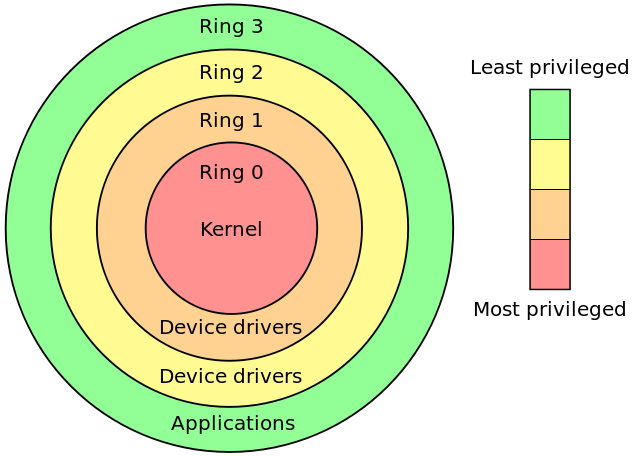
\includegraphics[scale=0.40]{rings.png}
  \caption{\label{fig:label} Anillos de protección, por Hertzsprung en Wikipedia}
\end{figure}
\vspace{1cm}

Entonces, `?en qué consiste la técnica que VMware utilizó en un primer momento para conseguir la virtualización de sistemas x86? Explicándolo de manera sencilla, consiste en ejecutar el sistema virtualizado en el anillo 1, y traduciendo el código no-virtualizable, a instrucciones que obtienen el mismo resultado en el hardware virtual. Dado el hecho de que el código de usuario resulta igual, éste se ejecuta directamente en el procesador para obtener más rendimiento.

Todo ésto en conjunto resulta en el sistema operativo completamente abstraído del hardware físico. A parte del aislamiento que así se obtiene, este método de virtualización no requiere ningún tipo de modificación en el sistema operativo para funcionar.

Algunos ejemplos de plataformas de virtualización completa son:

\begin{itemize}
    \item Parallels Workstation (Mac OS X)
    \item VMware Workstation (Windows, GNU/Linux)
    \item Oracle VM VirtualBox (Windows, Mac OS X, GNU/Linux)
\end{itemize}

\subsubsection{Paravirtualitzación}
\label{subsubsubsec:virt_para}

La paravirtualización es una técnica de emulación consistente en ofrecer una interfaz por software, que aunque no sea lo mismo que el hardware real, resulta bastante similar. El propósito de dicha interfaz es reducir el tiempo que el host virtualizado gasta realizando operaciones que resultan más complicadas de realizar en un entorno virtualizado comparado a un entorno normal. Esta técnica requiere que el sistema operativo virtualizado se haya portado a la API de paravirtualización, ya que un sistema en desconocimiento de ésta interfaz no puede hacerse funcionar bajo un software de paravirtualización.

En GNU/Linux la paravirtualitzación está disponible a partir de la versión 2.6.23 del kernel, y KVM puede utilizar la API VirtIO para virtualizar GNU/Linux, OpenBSD, FreeBSD, NetBSD, Plan 9 y Windows.

\subsubsection{Virtualitzación asistida por hardware}
\label{subsubsubsec:virt_hwassist}

La virtualización asistida por hardware se diferencia de la virtualización completa por el hecho de que consigue un mayor rendimiento gracias a la ayuda del hardware físico de la máquina anfitriona, principalmente el procesador. Ésto se basa en las siguientes teconologías:

\begin{itemize}
    \item En procesadores Intel, \textbf{Intel VT-x} (introducida por primera vez en los modelos 662 y 672 de Pentium 4 el 20 de noviembre de 2005), es la tecnología de virtualización x86 asistida por hardware ofrecida por Intel. Aunque a día de hoy todas las CPUs de Intel a excepción de modelos de bajo consumo y móviles soportan ésta teconología, en GNU/Linux se puede comprobar el soporte de la CPU actual mediante el siguiente comando: \texttt{cat /proc/cpuinfo | grep vmx}. A lo largo del tiempo Intel ha ido añadiendo nuevas funcionalidades a VT-x, siendo las maś importantes la adición de EPT para la emulación de tablas de página con la arquitectura Nehalem en 2008, el arranque del procesaodr lógico en modo real con la arquitectura Westmere en 2010, y el \emph{shadowing} de VMCS con Haswell en 2013.

    \item En procesadores AMD, \textbf{AMD-V} es la tecnología de virtualización asistida por hardware de AMD, introducida por primera vez con los Athlon 64, 64 FX y 64 X2 en 2006. 
\end{itemize}

Todo esto suena muy bien, pero cuando éstas tecnologías surgieron inicialmente, no ofrecían ventajas tangibles sobre la virtualización por software. Además, una estrategia exclusivamente de virtualización asistida por software implica bastantes trucos de implementación en la máquina virtual, provocando gran \emph{\gls{overhead}} de CPU, limitando la eficiencia de la máquina virtual.\@ Ésto se puede solventar mediante el uso de drivers paravirtualizados.

\subsubsection{Virtualitzación a nivel de sistema operativo}
\label{subsubsubsec:virt_containers}

También denominada virtualización de contenedores, este méodo permite al núcleo de un sistema operativo, ejecutar múltiples \emph{userspaces} por sí solo.

Este método no impone \emph{\gls{overhead}}\footnote{Véase el glosario}, dado que la interfaz de llamadas al sistema, o cualquier hardware, no necesita ser emulado. Por otro lado, ésto comporta que sólo se pueda virtualizar el mismo sistema operativo que la máquina anfitriona: mientras que cualquier sistema GNU/Linux puede emular otras distribuciones GNU/Linux, Windows y Mac OS X se ven limitados a emularse a ellos mismos.

Hoy en día las opciones más conocidas son \textbf{Docker}, y \textbf{LXC}.

\subsection{Arquitectura de oVirt}
\label{subsubsec:ovirt_arch}

\begin{figure}[ht!]
  \centering
  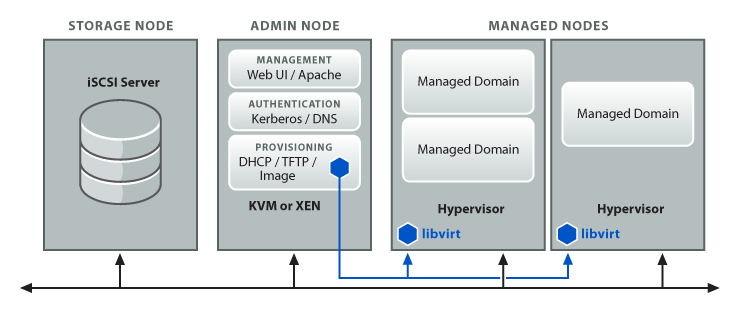
\includegraphics[scale=0.5]{ovirtarch.png}
  \caption{Arquitectura de oVirt}
\label{ovirtarch}
\end{figure}

oVirt consta de una arquitectura relativamente simple, en la cual encontramos al menos \textbf{dos} máquinas:

\begin{itemize}
    \item Un nodo de control: Esta es la máquina donde se instala el oVirt Engine. Desde aquí realizaremos todas tareas de administración y mantenimiento del \emph{datacenter}: despliegue y migración de máquinas virtuales monitorización de los hosts, configuración del almacenamiento, y más.

    \item Hosts de virtualización: Aquí es dónde se ejecutarán las máquinas virtuales. Éstos han de disponer de una CPU con las extensiones de virtualización mencionadas en la sección anterior.
\end{itemize}

La imagen especifica también un tercer nodo: el de almacenamiento. Aquí es donde se guardan tanto las imágenes ISO de instalación de sistemas operativos, como las imágenes de discos duros en uso por las máquinas virtuales. Éste puede ser tanto un host dedicado como en la imagen, o integrarse en el nodo de administración. oVirt soporta diferentes soluciones de almacenamiento en red, como NFS, iSCSI o GlusterFS.\@

Como se ve en la imagen, el nodo de administración y los hosts de virtualización utilizan la API \textbf{libvirt}, para realizar todo el trabajo con máquinas virtuales en materia de creación, arranque y control del almacenamiento. Respecto a la forma de virtualizar, podemos decir que libvirt y KVM virtualizan la máquina virtual por completo, ayudándose de la paravirtualización y las extensiones de virtualización presentes en el procesador.

\section{Requisitos}
\label{subsec:requisitios}

\subsection{Hardware}
\label{subsubsec:hardware}

Los siguientes son las características recomendadas para instalaciones pequeñas y medias, de los diferentes host que forman parte de la arquitectura de oVirt:

\begin{itemize}
\item oVirt Engine
  \begin{itemize}
  \item CPU de dos núcleos.
  \item 4 GB de RAM.\@
  \item 25 GB de espacio libre en el disco duro.
  \item Interfaz de red de 1 Gbps.
  \end{itemize}
\item Hosts de virtualización
  \begin{itemize}
  \item CPU de dos núcleos con extensiones de virtualización (Intel VT-x / AMD-V)
  \item 10 GB de RAM
  \item 10 GB de espacio libre en el disco duro.
  \item Interfaz de red de 1 Gbps.
  \end{itemize}
\end{itemize}

Las máquinas utilizadas para los host de virtualización en éste proyecto, por razones estrictamente monetarias, son un par de Acer Aspire X, con las siguientes especificaciones:

\begin{itemize}
    \item Intel Pentium J29000 (Quad Core, 2,41 GHz)
    \item 4 GB de RAM
    \item 500 GB HD
    \item Interfaz Gigabit Ethernet
\end{itemize}

Obviamente, éstos quedan muy por debajo de los recomendados incluso para instalaciones pequeñas, por lo que éste proyecto no debe considerarse apto para ser llevado a cabo en producción, al menos en su estado actual.

\subsection{Software}
\label{subsubsec:software}

La siguiente lista muestra los sistemas operativos que oVirt soport a la hora de ser virtualizados:

\begin{itemize}
    \item Windows (XP, 7, 8, 2003, 2008, 2012)
    \item RHEL 5, 6 o 7
    \item CentOS 5, 6 o 7
    \item Fedora 16 - 23.
    \item Ubuntu 12.04 + 
    \item openSUSE 12.x+
\end{itemize}

